\chapter{Simplifying the Construction of Optimisation Heuristics}
\label{chap:deeptune}


\section{Introduction}

There are countless scenarios during the compilation and execution of a program where decisions must be made as to how, or if, a particular optimisation should be applied. Modern compilers and runtimes are rife with hand-coded \emph{heuristics} which perform this decision making. The performance of programs is thus dependent on the quality of these heuristics.

Handwritten heuristics require expert knowledge, take a lot of time to construct, and in many cases lead to sub-optimal decisions. Researchers have focused on machine learning as a means of constructing high-quality heuristics that often outperform their handcrafted equivalents~\cite{Micolet2016,Falch2015,Stephenson2005,Agakov,Cummins2016a}. A \emph{predictive model} is trained, using supervised machine learning, on empirical performance data and important quantifiable properties, or \emph{features}, of representative programs. The model learns the correlation between these features and the optimisation decision that maximises performance. The learned correlations are used to predict the best optimisation decisions for new programs. Previous works in this area were able to build machine learning based heuristics with less effort, that outperform ones created manually by experts~\cite{Grewe2013,Magni2014}.

Still, experts are not completely removed from the design process, which is shown in Figure~\ref{fig:overview-a}. Selecting the appropriate features is a manual undertaking which requires a deep understanding of the system. The designer essentially decides which compile or runtime characteristics affect optimisation decisions and expresses them in ways that make it easy to model their relationship to performance. Failing to identify an important feature has a negative effect on the resulting heuristic. For example, in Section~\ref{subsec:eval-extended} the \citeauthor{Grewe2013} model is shown to be missing one such feature, causing performance to be 40\% lower on average.

To make heuristic construction fast and cheap, humans must be taken out of the loop. While techniques for automatic feature generation from the compiler IR have been proposed in the past~\cite{Namolaru2010a,Leather2014}, they do not solve the problem in a practical way. They are deeply embedded into the compiler, require expert knowledge to guide the generation, have to be repeated from scratch for every new heuristic, and their search time can be prohibitive. Inspired by the astounding success of recurrent neural networks at generating program code for benchmarking and compiler testing, I hypothesised that a learning system should be able to automatically extract feature representations from source code. These learned feature representations could then be used as inputs to other learning systems for task-specific purposes such as learning optimisation heuristics. This would mitigrate the \emph{feature design} challenge (Section~\ref{subsec:challenge-features}).

The experiments showed that this was a conservative target: with deep neural networks, one can entirely bypass static feature extraction and learn optimisation heuristics directly on raw code, without the need for an intermediate representation.

\begin{figure}[t!]
  \centering
  \subfloat[Current state-of-practice]{%
    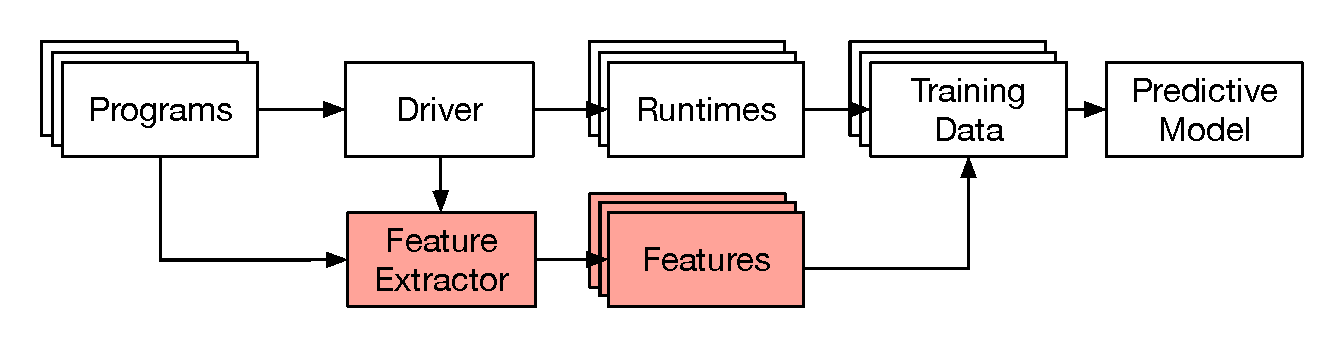
\includegraphics[width=.95\columnwidth]{img/training_model_a}%
    \label{fig:overview-a}%
  }\\*%
  \subfloat[The proposed approach]{%
    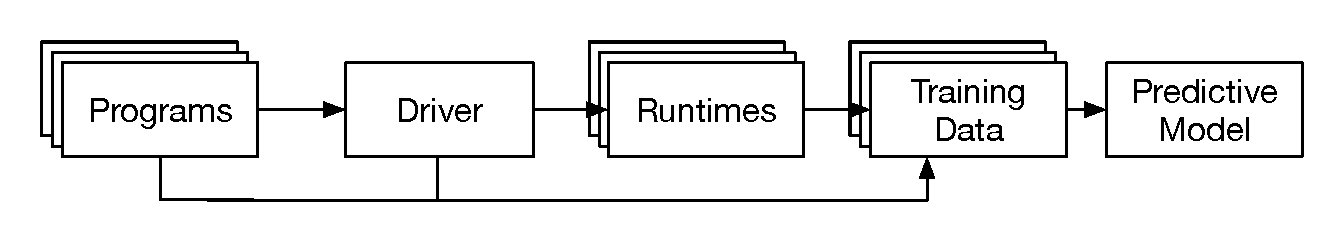
\includegraphics[width=.95\columnwidth]{img/training_model_b}%
    \label{fig:overview-b}%
  }%
  \caption[Using machine learning for compiler optimisations]{%
    Building a predictive model. The model is originally trained on performance data and features extracted from the source code and the runtime behaviour. The proposed approach bypasses feature extraction, instead learning directly over raw program source code.%
  }%
  \label{fig:overview}
\end{figure}

Figure~\ref{fig:overview-b} shows the proposed methodology. Instead of manually extracting features from input programs to generate training data, program code is used directly as training data. Programs are fed through a series of artificial neural networks which learn how code correlates with performance. Internally and without prior knowledge, the networks construct complex abstractions of the input program characteristics and correlations between those abstractions and performance. This chapter proposes replacing the need for compile-time or static code features, merging feature and heuristic construction into a single process of joint learning. The system admits auxiliary features to describe information unavailable at compile time, such as the sizes of runtime input parameters. Beyond these optional inclusions, the system is able to learn optimisation heuristics without human guidance.

By employing \emph{transfer learning}~\cite{Yosinski2014}, the proposed approach is able to produce high-quality heuristics even when learning on a small number of programs. The properties of the raw code that are abstracted by the beginning layers of the artificial neural networks are mostly independent of the optimisation problem. Parts of the network may be reused across heuristics, and, in the process, speed up learning considerably.

The approach is evaluated on two parallel compilation problems: heterogeneous device mapping and GPU thread coarsening. Good heuristics for these two problems are important for extracting performance from heterogeneous systems, and the fact that machine learning has already been applied to constructing heuristics for these problems allows direct comparison. Prior machine learning approaches resulted in good heuristics which extracted 73\% and 79\% of the available performance respectively but required extensive human effort to select the appropriate features. Nevertheless, the approach presented in this chapter was able to outperform them by 14\% and 12\%, which indicates a better identification of important program characteristics, without any expert help.

This chapter is organised as follows: Section~\ref{sec:deeptune} describes DeepTune, a novel system for building optimisation heuristics. In Sections~\ref{sec:deeptune-case-study-a} and~\ref{sec:deeptune-case-study-b}, case studies are presented that evaluate DeepTune's capabilities first at predicting heterogeneous device mapping, then thread coarsening. Section~\ref{sec:deeptune-transfer-learning} explores the novel transfer of information between the two problems. Section~\ref{sec:deeptune-internal-states} illuminates the inner workings of DeepTune by analysing the internal state within the artificial neural networks. Finally, Section~\ref{sec:deeptune-conclusion} contains concluding remarks.


\section{DeepTune: Learning On Raw Program Code}%
\label{sec:deeptune}

DeepTune is an end-to-end machine learning pipeline for optimisation heuristics. Its primary input is the source code of a program to be optimised, and through a series of artificial neural networks, it directly predicts the optimisation which should be applied. By learning on source code, the approach is not tied to a specific compiler, platform, or optimisation problem. The same design can be reused to build multiple heuristics. The most important innovation of DeepTune is that it obviates the need for human experts to select and tune appropriate features.


\subsection{Overview}

Figure~\ref{fig:deeptune} provides an overview of the system. A source re-writer removes semantically irrelevant information (such as comments) from the source code of the target program and passes it to a language model. The language model converts the arbitrary length stream of code into a fixed length vector of real values which fully capture the properties and structure of the source, replacing the role of hand-designed features. This vector can then optionally be concatenated with auxiliary inputs, which allow passing additional data about runtime or architectural parameters to the model for heuristics which need more than just compile-time information. Finally, a standard feed-forward network is used to predict the best heuristic parameters to optimise the program.

\begin{figure}
  \centering
  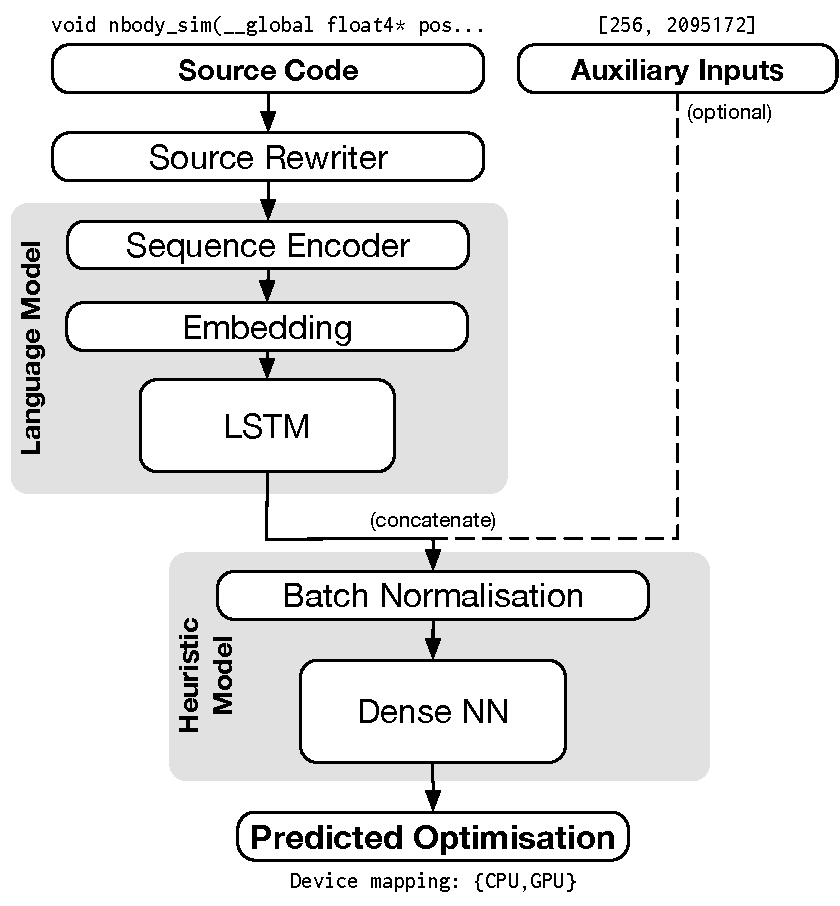
\includegraphics[width=.85\columnwidth]{img/deeptune} %
  \caption[DeepTune system overview]{%
    DeepTune system overview. Code properties are extracted from source code by the
    language model. They are fed, together with optional auxiliary inputs, to
    the heuristic model to produce the final prediction.%
  }%
  \label{fig:deeptune}
\end{figure}

DeepTune is open source. The model is implemented in Keras, with TensorFlow~\cite{Abadi} and Theano~\cite{Bergstra2011} back-ends.


\subsection{Language Model}

Learning effective representations of source code is a difficult task. A successful model must be able to:

\begin{itemize}
  \item derive semantic and syntactic patterns of a programming language entirely from sample codes;
  \item identify the patterns and representation in source codes which are relevant to the task at hand; and
  \item discriminate performance characteristics arising from potentially subtle differences in similar codes.
\end{itemize}

To achieve this task, state-of-the-art language modelling techniques are employed, coupled with a series of generic, language-agnostic code transformations.

\subsubsection{Source Re-writer}

To begin with, a series of \emph{source normalising} transformations are applied, extending the system described in Chapter~\ref{chap:deepsmith}. These transformations, implemented as an LLVM pass, parse the AST, removing conditional compilation, then rebuild the input source code using a consistent code style and identifier naming scheme. The role of source normalisation is to simplify the task of modelling source code by ensuring that trivial semantic differences in programs such as the choice of variable names or the insertion of comments do not affect the learned model. Figures~\ref{subfig:source_in} and~\ref{subfig:source_out} show the source rewriting process applied to a simple program.

\subsubsection{Sequence Encoder}

The textual representation of program codes must be encoded as numeric sequences for feeding as input to the machine learning model. This is achieved by extending the encoder described in Section~\ref{sec:deepsmith}, in which a programming language's keywords and common names are treated as individual tokens while the rest of the text is encoded on a character-level basis. This approach hits a balance between compressing the input text and keeping the number of tokens in the vocabulary low. Figure~\ref{subfig:source_vocab} shows the vocabulary derived from the single input source code in Figure~\ref{subfig:source_out}.

\subsubsection{Embedding}

During encoding, tokens in the vocabulary are mapped to unique integer values, e.g. \texttt{float} $\rightarrow 0$, \texttt{int} $\rightarrow$ 1. The chosen integer values are arbitrary, and offer a \emph{sparse} data representation, meaning that a language model cannot infer the relationships between tokens based on their mappings. This is in contrast to the \emph{dense} representations of other domains, such as pixels in images, which can be interpolated between to derive the differences in colours.

To mitigate this, an \emph{embedding} is used, which translates tokens in a sparse, integer-encoded vocabulary into a lower dimensional vector space, allowing semantically related tokens like \texttt{float} and \texttt{int} to be mapped to nearby points~\cite{Mikolov2013a,Baroni2014}. An embedding layer maps each token in the integer-encoded vocabulary to a vector of real values. Given a vocabulary size $|V|$ and embedding dimensionality $D$, an embedding matrix $\bm{W_{E}} \in \mathbb{R}^{|V| \times D}$ is learned during training such that an integer-encoded sequence of tokens $\bm{t} \in \mathbb{N}^{L}$ is mapped to the matrix $\bm{T} \in \mathbb{R}^{L \times D}$. In this work, a embedding dimensionality $D = 64$ is used, selected somewhat arbitrarily, with best-practices suggesting an empirical approach to determine good values. Research into analytical models for selecting embedding dimensionality is ongoing~\cite{Yin2018a,Naumov2019}.

\newsavebox{\NvidiaStreamClusterInput}
\begin{lrbox}{\NvidiaStreamClusterInput}
  \begin{minipage}{\textwidth}
    \begin{minted}{opencl_lexer.py:OpenCLLexer -x}
kernel void memset_kernel(global char * mem_d, short val, int number_bytes){
    const int thread_id = get_global_id(0);
    mem_d[thread_id] = val; }
    \end{minted}
  \end{minipage}
\end{lrbox}

\newsavebox{\NvidiaStreamClusterOutput}
\begin{lrbox}{\NvidiaStreamClusterOutput}
  \begin{minipage}{\textwidth}
    \begin{minted}{opencl_lexer.py:OpenCLLexer -x}
kernel void A(global char* a, short b, int c) {
  const int d = get_global_id(0);
  a[d] = b;
}
    \end{minted}
  \end{minipage}
\end{lrbox}

\begin{figure}
  \centering %
  \subfloat[%
    An example, short OpenCL kernel, taken from Nvidia's \emph{streamcluster}.%
  ]{%
    \noindent\mbox{\parbox{\columnwidth}{\usebox{\NvidiaStreamClusterInput}}}%
    \label{subfig:source_in}%
  }\\%
  \subfloat[%
    The \emph{streamcluster} kernel after source rewriting. Variable and
    function names are normalised, comments removed, and code style enforced.%
  ]{%
    \noindent\mbox{\parbox{\columnwidth}{\usebox{\NvidiaStreamClusterOutput}}}%
    \label{subfig:source_out}%
  }\\%
  \subfloat[%
    Derived vocabulary, ordered by their appearance in the
    input~\protect\subref{subfig:source_out}. The vocabulary maps tokens to
    integer indices.%
  ]{%
    \footnotesize
\begin{tabular}{l l | l l | l l}
  \toprule
  \textbf{idx} & \textbf{token} & \textbf{idx} & \textbf{token} & \textbf{idx} & \textbf{token} \\
  \midrule
  \texttt{1} & \texttt{`\_\_kernel'} & \texttt{10} & \texttt{`,'} & \texttt{19} & \texttt{`const'} \\
  \texttt{2} & \texttt{` '} & \texttt{11} & \texttt{`short'} & \texttt{20} & \texttt{`d'} \\
  \texttt{3} & \texttt{`void'} & \texttt{12} & \texttt{`b'} & \texttt{21} & \texttt{`='} \\
  \texttt{4} & \texttt{`A'} & \texttt{13} & \texttt{`int'} & \texttt{22} & \texttt{`get\_global\_id'} \\
  \texttt{5} & \texttt{`('} & \texttt{14} & \texttt{`c'} & \texttt{23} & \texttt{`0'} \\
  \texttt{6} & \texttt{`\_\_global'} & \texttt{15} & \texttt{`)'} & \texttt{24} & \texttt{`;'} \\
  \texttt{7} & \texttt{`char'} & \texttt{16} & \texttt{`\{'} & \texttt{25} & \texttt{`['} \\
  \texttt{8} & \texttt{`*'} & \texttt{17} & \texttt{`\textbackslash n'} & \texttt{26} & \texttt{`]'} \\
  \texttt{9} & \texttt{`a'} & \texttt{18} & \texttt{`\space\space'} & \texttt{27} & \texttt{`\}'} \\
  \bottomrule
\end{tabular}%
%
    \label{subfig:source_vocab}%
  }\\%
  \subfloat[%
    Indices encoded kernel sequence. Sequences may be padded to a fixed length
    by repeating an out-of-vocabulary integer (e.g. -1).%
  ]{%
    \rowcolors{2}{white}{gray!25}
\begin{tabular}{l l l l l l l l l l l}
	\toprule
	\texttt{01} & \texttt{02} & \texttt{03} & \texttt{02} & \texttt{04} & \texttt{05} & \texttt{06} & \texttt{02} & \texttt{07} & \texttt{08} & \texttt{02} \\
	\texttt{09} & \texttt{10} & \texttt{02} & \texttt{11} & \texttt{02} & \texttt{12} & \texttt{10} & \texttt{02} & \texttt{13} & \texttt{02} & \texttt{14} \\
	\texttt{15} & \texttt{02} & \texttt{16} & \texttt{17} & \texttt{18} & \texttt{19} & \texttt{02} & \texttt{13} & \texttt{02} & \texttt{20} & \texttt{02} \\
	\texttt{21} & \texttt{02} & \texttt{22} & \texttt{05} & \texttt{23} & \texttt{15} & \texttt{24} & \texttt{17} & \texttt{18} & \texttt{09} & \texttt{25} \\
	\texttt{20} & \texttt{26} & \texttt{02} & \texttt{21} & \texttt{02} & \texttt{12} & \texttt{24} & \texttt{17} & \texttt{27} & \multicolumn{2}{l}{\texttt{<pad\ldots>}} \\
	\bottomrule
\end{tabular}
%
    \label{subfig:source_enc}%
  }%
  \caption[Deriving a vocabulary encoding from source code]{%
    Deriving a tokenised $1$-of-$k$ vocabulary encoding from source
    code.%
  }%
  \label{fig:encoding}%
\end{figure}


\subsubsection{Sequence Characterisation}

Once source codes have been encoded into sequences of embedding vectors, artificial neural networks are used to extract a fixed size vector which characterises the entire sequence. This is comparable to the hand engineered feature extractors used in prior works, but is a \emph{learned} process that occurs entirely --- and automatically --- within the hidden layers of the network.

The Long Short-Term Memory (LSTM) architecture is used for sequence characterisation~\cite{Hochreiter1997}. LSTMs implement a Recurrent Neural Network in which the activations of neurons are learned with respect not just to their current inputs, but to previous inputs in a sequence. Unlike regular recurrent networks in which the strength of learning decreases over time (a symptom of the \emph{vanishing gradients} problem~\cite{Pacanu2013}), LSTMs employ a \emph{forget gate} with a linear activation function, allowing them to retain activations for arbitrary durations. This makes them effective at learning complex relationships over long sequences~\cite{Lipton2015}, an especially important capability for modelling program code, as dependencies in sequences frequently occur over long ranges (for example, a variable may be declared as an argument to a function and used throughout).

The LSTM network has two layers of cells. The network receives a sequence of embedding vectors, and returns a single output vector, characterising the entire sequence.


\subsection{Auxiliary Inputs}

An arbitrary number of additional real-valued \emph{auxiliary inputs} may be optionally used to augment the source code input. These inputs are provided as a means of increasing the flexibility of the system, for example, to support applications in which the optimisation heuristic depends on dynamic values which cannot be statically determined from the program code~\cite{Ding2015,Stephenson2005}. When present, the values of auxiliary inputs are concatenated with the output of the language model and fed into a heuristic model.


\subsection{Heuristic Model}

The heuristic model takes the learned representations of the source code and auxiliary inputs (if present) and uses these values to make the final optimisation prediction.

First, the values are normalised. Normalisation is necessary because the auxiliary inputs can have any values, whereas the language model activations are in the range [0,1]. If the heuristic model inputs were not normalised, then scaling the auxiliary inputs could affect the training of the heuristic model. Normalisation occurs in batches. The batch normalisation method of~\cite{Ioffe2015a} is used, in which each scalar of the heuristic model's $n$ inputs $\bm{x}^{(1)}, \ldots, \bm{x}^{(n)}$ is independently normalised to a mean 0 and standard deviation of 1:

\begin{equation}
\bm{\hat{x}}^{(i)} = \bm{\upgamma}^{(i)} \frac{\bm{x}^{(i)} - E(\bm{x}^{(i)})}{\sqrt{Var(\bm{x}^{(i)})}} + \bm{\beta}^{(i)}
\end{equation}

Where $\bm{\upgamma}$ and $\bm{\beta}$ are scale and shift parameters, learned during training.

The final component of DeepTune is comprised of two fully connected artificial neural network layers. The first layer consists of 32 neurons. The second layer consists of a single neuron for each possible heuristic decision. Each neuron applies an activation function $\phi(z)$ over its inputs. Rectified linear units $\phi(z) = max(z, 0)$ are used in the first layer due to their improved performance during the training of deep networks~\cite{Nair2010}. For the output layer, sigmoid activation functions $\phi(z) = \frac{1}{1 + e^{-z}}$ are used which provide activations in the range $[0,1]$.

The activation of each neuron in the output layer represents the model's confidence that the corresponding decision is the correct one. Taking the $\argmax$ of the output layer produces the decision with the largest activation. For example, for a binary optimisation heuristic the final layer will consist of two neurons, and the predicted optimisation is the neuron with the largest activation.


\subsection{Training the Network}

DeepTune is trained in the same manner as prior supervised machine learning works, the key difference being that instead of having to manually create and extract features from programs, the raw program codes themselves are used.

The model is trained with Stochastic Gradient Descent (SGD) using the Adam optimiser~\cite{Kingma2015}. For training data $\bm{x}^{(1)}, \ldots, \bm{x}^{(n)}$, SGD attempts to find the model parameters $\bm{\hat{\Theta}}$ that minimise the output of a loss function:

\begin{equation}
\bm{\hat{\Theta}} = \argmin_{\bm{\Theta}} \frac{1}{n} \sum_{i=1}^{n} \mathcal{L} \left( \bm{x}^{(i)}, \bm{\Theta} \right)
\end{equation}

where loss function $\mathcal{L} \left(\bm{x}, \bm{\Theta} \right)$ computes the logarithmic difference between the predicted and expected values given a model constructed using parameters $\bm{\Theta}$.

To reduce training time, multiple inputs are \emph{batched} together and fed into the artificial neural network simultaneously, reducing the frequency of costly weight updates during back-propagation. This requires that the inputs to the language model be the same length. Sequences are padded up to a fixed length of 1024 tokens using a special out-of-vocabulary padding token $\tau \not\in V$, allowing matrices of \texttt{batch\_size} $\times$ \texttt{max\_seq\_len} tokens to be processed simultaneously. Batching and padding sequences to a maximum length is only to improve training time. In production use, sequences do not need to be padded, allowing classification of arbitrary length codes in linear time.


\section{Case Study A: OpenCL Heterogeneous Mapping}
\label{sec:deeptune-case-study-a}

OpenCL provides a platform-agnostic framework for heterogeneous parallelism. This allows a program written in OpenCL to execute transparently across a range of different devices, from CPUs to GPUs and FPGAs. Given a program and a choice of execution devices, the question then is on which device should one execute the program to maximise performance?


\subsection{State-of-the-art}

I return to the \citeauthor{Grewe2013}~\cite{Grewe2013} predictive model of Chapter~\ref{chap:clgen} for mapping OpenCL kernels to the optimal device in CPU/GPU heterogeneous systems. The authors use supervised learning to construct decision trees, using a combination of static and dynamic kernel features. The static program features are extracted using a custom LLVM pass; the dynamic features are taken from the OpenCL runtime.


\paragraph*{Expert Chosen Features}

Table~\ref{tab:grewe-features-final} shows the features used in their work. Each feature is an expression built upon the code and runtime metrics given in Table~\ref{tab:grewe-features-raw}.

\begin{table}
  \rowcolors{2}{gray!25}{white}
  \centering%
  \subfloat[Feature values]{
    \begin{tabular}{| l L{4.5cm} |}
      \hline
      \rowcolor{gray!50}
      \textbf{Name} & \textbf{Description} \\
      \hline
      \texttt{F1: data size/(comp+mem)} & commun.-computation ratio \\
      \texttt{F2: coalesced/mem} & \% coalesced memory accesses \\
      \texttt{F3: (localmem/mem)$\times$wgsize} & ratio local to global mem accesses  $\times$ \#.\ work-items \\
      \texttt{F4: comp/mem} & computation-mem ratio\\
      \hline
    \end{tabular}%
    \label{tab:grewe-features-final}%
  }\\ %
  \subfloat[Values used in feature computation]{%
    \rowcolors{2}{gray!25}{white}
    \begin{tabular}{| l c l |}
    	\hline
      \rowcolor{gray!50}
      \textbf{Name} & \textbf{Type} & \textbf{Description} \\
      \hline
      \texttt{comp} & static & \#.\ compute operations \\
      \texttt{mem} & static & \#.\ accesses to global memory \\
      \texttt{localmem} & static & \#.\ accesses to local memory \\
      \texttt{coalesced} & static & \#.\ coalesced memory accesses \\
      \texttt{data size} & dynamic & size of data transfers \\
      \texttt{work-group size} & dynamic & \#.\ work-items per kernel \\
      \hline
    \end{tabular}%
    \label{tab:grewe-features-raw}%
  }
  \caption[Heterogeneous mapping model features]{%
    Features used by \emph{Grewe et al. }to predict heterogeneous device
    mappings for OpenCL kernels.%
  } %
  \label{tab:grewe-features} %
\end{table}



\subsection{Experimental Setup}

The predictive model of \citeauthor{Grewe2013}~\cite{Grewe2013} is replicated. The same experimental setup is used as in Chapter~\ref{chap:clgen} in which the experiments are extended to a larger set of 71 programs, summarised in Table~\ref{tab:cgo-benchmarks}. The programs are evaluated on two CPU-GPU platforms, detailed in Table~\ref{tab:cgo-platforms}.

\begin{table}
  \centering%
  \rowcolors{2}{gray!25}{white}
  \begin{tabular}{| l r r r |}
    \hline
    \rowcolor{gray!50}
    & \textbf{Version} & \textbf{\#. benchmarks} & \textbf{\#. kernels}\\
    \hline
    \textbf{NPB (SNU~\cite{Seo2011})} & 1.0.3 & 7 & 114 \\
    \textbf{Rodinia~\cite{Che2009}} & 3.1 & 14 & 31 \\
    \textbf{NVIDIA SDK} & 4.2 & 6 & 12 \\
    \textbf{AMD SDK} & 3.0 & 12 & 16 \\
    \textbf{Parboil~\cite{Stratton2012}} & 0.2 & 6 & 8 \\
    \textbf{PolyBench~\cite{Grauer-Gray2012}} & 1.0 & 14 & 27 \\
    \textbf{SHOC~\cite{Danalis2010}} & 1.1.5 & 12 & 48 \\
    \textbf{Total} & - & 71 & 256 \\
    \hline
  \end{tabular}
  \caption[Benchmarks used in Case Study A]{%
    Benchmarks used in Case Study A.%
  }
  \label{tab:cgo-benchmarks}
\end{table}

\begin{table}[t!]
  \centering %
    \rowcolors{2}{gray!25}{white}
    \begin{tabular}{| l l l l| }
      \hline
      \rowcolor{gray!50}
      & \textbf{Frequency} & \textbf{Memory} & \textbf{Driver} \\
      \hline
      \textbf{Intel Core i7-3820} & 3.6 GHz & 8GB & AMD 1526.3 \\
      \textbf{AMD Tahiti 7970} & 1000 MHz & 3GB & AMD 1526.3 \\
      \textbf{NVIDIA GTX 970} & 1050 MHz & 4GB & NVIDIA 361.42 \\
      \hline
    \end{tabular}
    \caption[Benchmarks used in Case Study A]{%
    Experimental platforms used in Case Study A.%
    }
    \label{tab:cgo-platforms}
\end{table}


\paragraph*{DeepTune Configuration}

Figure~\ref{fig:nn}a shows the artificial neural network configuration of DeepTune for the task of predicting optimal device mapping. The OpenCL kernel source code is used as input, along with the two dynamic values \emph{work-group size} and \emph{data size} available to the OpenCL runtime.


\paragraph*{Model Evaluation}

\emph{Stratified 10-fold cross-validation} is used to evaluate the quality of the predictive models~\cite{Han2011}. Each program is randomly allocated into one of 10 equally-sized sets; the sets are balanced to maintain a distribution of instances from each class consistent with the full set. A model is trained on the programs from all but one of the sets, then tested on the programs of the unseen set. This process is repeated for each of the 10 sets to construct a complete prediction over the whole data set.

\begin{figure}[t!]
  \centering
  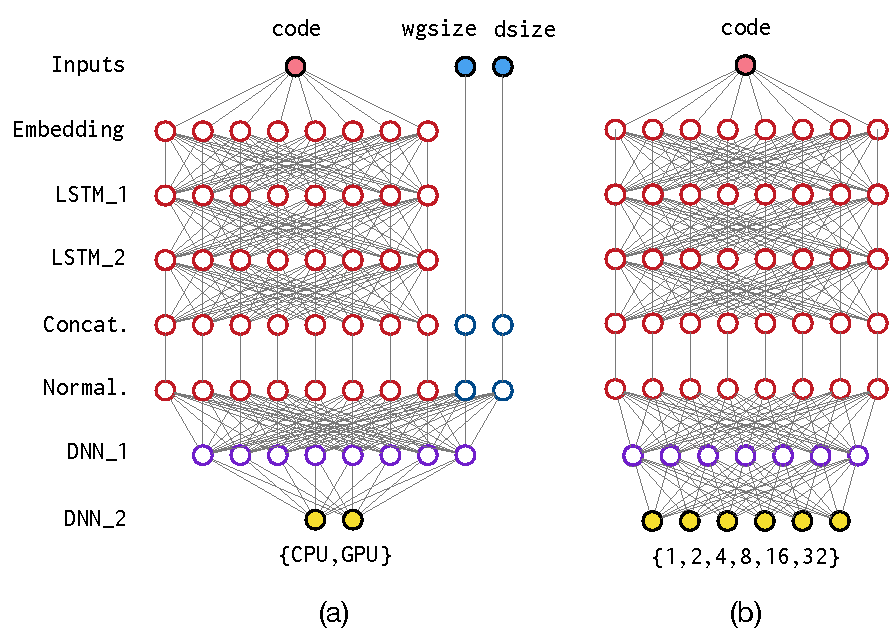
\includegraphics[width=\columnwidth]{img/nn} %
  \caption[DeepTune artificial neural networks]{%
    DeepTune artificial neural networks, configured for (a) heterogeneous mapping, and (b) thread coarsening factor. The design stays almost the same regardless of the optimisation problem. The only changes are the extra input for (a) and size of the output layers. To aid in visualisation, the number of neurons in each layer is reduced. For the true neuron counts, see Table~\ref{tab:nn-size}%
  }%
  \label{fig:nn}
\end{figure}


\subsection{Experimental Results}

Selecting the optimal execution device for OpenCL kernels is essential for maximising performance. For a CPU/GPU heterogeneous system, this presents a binary choice. In this experiment, the approach is compared to a static single-device approach and the \citeauthor{Grewe2013} predictive model. The \emph{static mapping} selects the device which gave the best average case performance over all the programs. On the AMD platform, the best-performing device is the CPU; on the NVIDIA platform, it is the GPU.

Figure~\ref{fig:cgo-accuracy} shows the accuracy of both predictive models and the static mapping approach for each of the benchmark suites. The static approach is accurate for only 58.8\% of cases on AMD and 56.9\% on NVIDIA. This suggests the need for choosing the execution device on a per program basis. The \citeauthor{Grewe2013} model achieves an average accuracy of 73\%, a significant improvement over the static mapping. By automatically extracting useful feature representations from the source code, DeepTune gives an average accuracy of 82\%, an improvement over both schemes.

\begin{figure}
  \centering %
  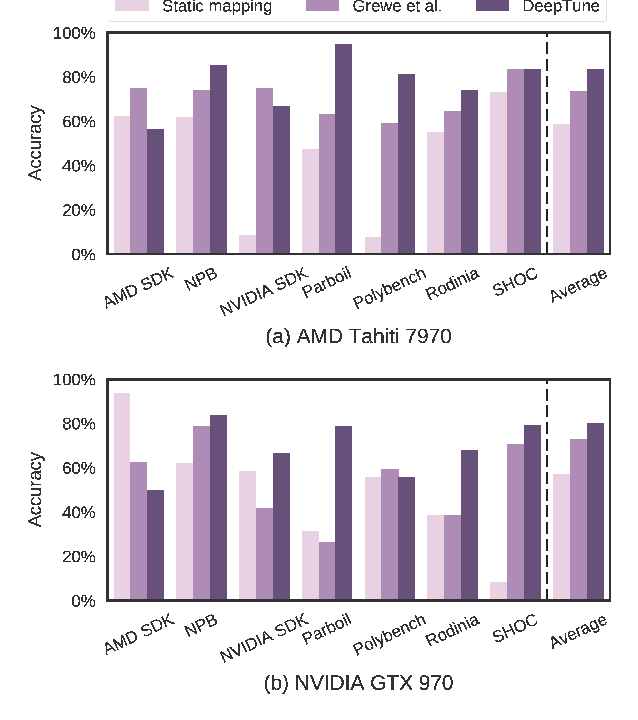
\includegraphics[width=.85\columnwidth]{img/cgo-acc}%
  \caption[Accuracy of optimisation heuristics for heterogeneous device mapping]{%
    Accuracy of optimisation heuristics for heterogeneous device mapping, aggregated by benchmark suite. The optimal static mapping achieves 58\% accuracy. The \citeauthor{Grewe2013} and DeepTune predictive models achieve accuracies of 73\% and 84\%, respectively.%
  }
  \label{fig:cgo-accuracy}
\end{figure}

Using the static mapping as a baseline, the relative performance of each program is computed using the device selected by the \citeauthor{Grewe2013} and DeepTune models. Figure~\ref{fig:cgo-speedup} shows these speedups. Both predictive models significantly outperform the static mapping; the Grewe \emph{et al.\ }model achieves an average speedup of $2.91\times$ on AMD and $1.26\times$ on NVIDIA (geometric mean $1.18\times$). In 90\% of cases, DeepTune matches or outperforms the predictions of the Grewe \emph{et al.\ }model, achieving an average speedup of $3.34\times$ on AMD and $1.41\times$ on NVIDIA (geometric mean $1.31\times$). This 14\% improvement in performance comes at a greatly reduced cost, requiring no intervention by humans.


\begin{figure}
  \centering %
  \subfloat[][AMD Tahiti 7970]{%
    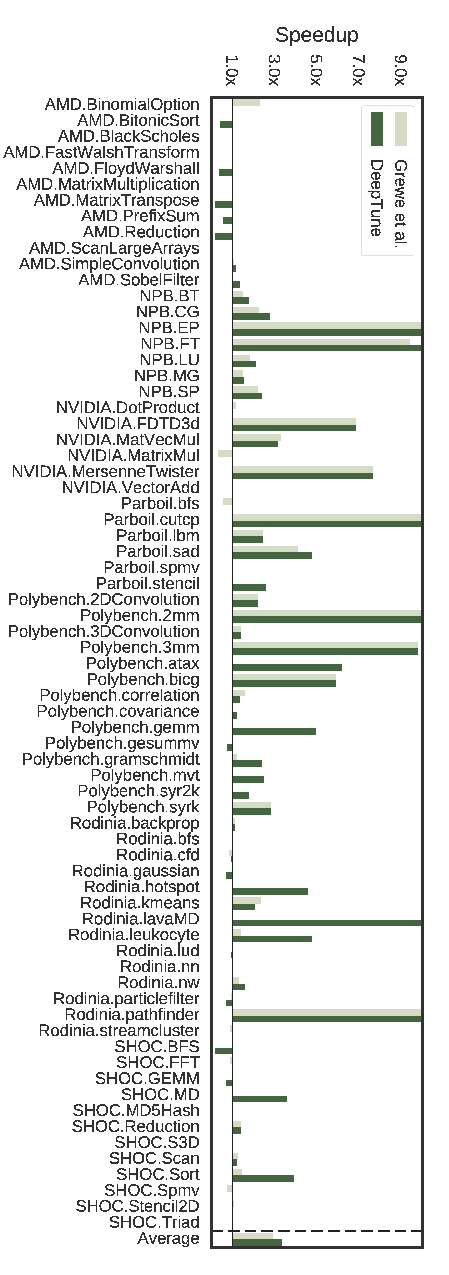
\includegraphics[width=.48\textwidth]{img/cgo-speedup-amd}%
    \label{fig:cgo-speedup-amd}}%
  \subfloat[][NVIDIA GTX 970]{%
    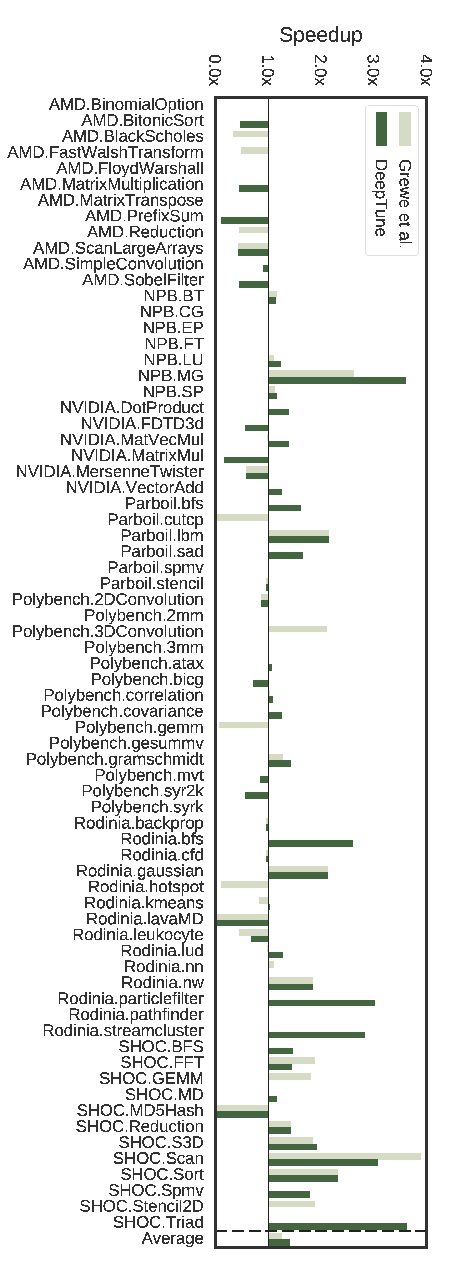
\includegraphics[width=.48\textwidth]{img/cgo-speedup-nvidia}%
    \label{fig:cgo-speedup-nvidia}}%
  \caption[Speedup of predicted heterogeneous mappings]{%
    Speedup of predicted heterogeneous mappings over the best static mapping for both platforms. In~\subref{fig:cgo-speedup-amd}, DeepTune achieves an average speedup of 3.43x over static mapping and 18\% over \citeauthor{Grewe2013}. In~\subref{fig:cgo-speedup-nvidia}, the speedup is 1.42x and 13\% respectively.%
  }
  \label{fig:cgo-speedup}
\end{figure}


\section{Case Study B: OpenCL Thread Coarsening Factor}
\label{sec:deeptune-case-study-b}

Thread coarsening is an optimisation for parallel programs in which the operations of two or more threads are fused together. The number of threads which must be executed is then reduced by this thread coarsening factor. This optimisation might prove beneficial on certain combinations of programs and architectures, for example, programs with a large potential for Instruction-level Parallelism on Very Long Instruction Word architectures.


\subsection{State-of-the-art}

\citeauthor{Magni2014} present a predictive model for OpenCL thread coarsening in~\cite{Magni2014}. They implement an iterative heuristic which determines whether a given program would benefit from coarsening. If yes, then the program is coarsened, producing a new program from which features can be computed. This process is repeated, allowing further coarsening. In this manner, the problem is reduced from a multi-label classification problem into a series of binary decisions, shown in Figure~\ref{fig:cf-magni}. They select from one of six possible coarsening factors: $(1, 2, 4, 8, 16, 32)$, divided into 5 binary choices.

\begin{figure}
  \centering %
  \subfloat[\citeauthor{Magni2014} cascading binary model.]{%
    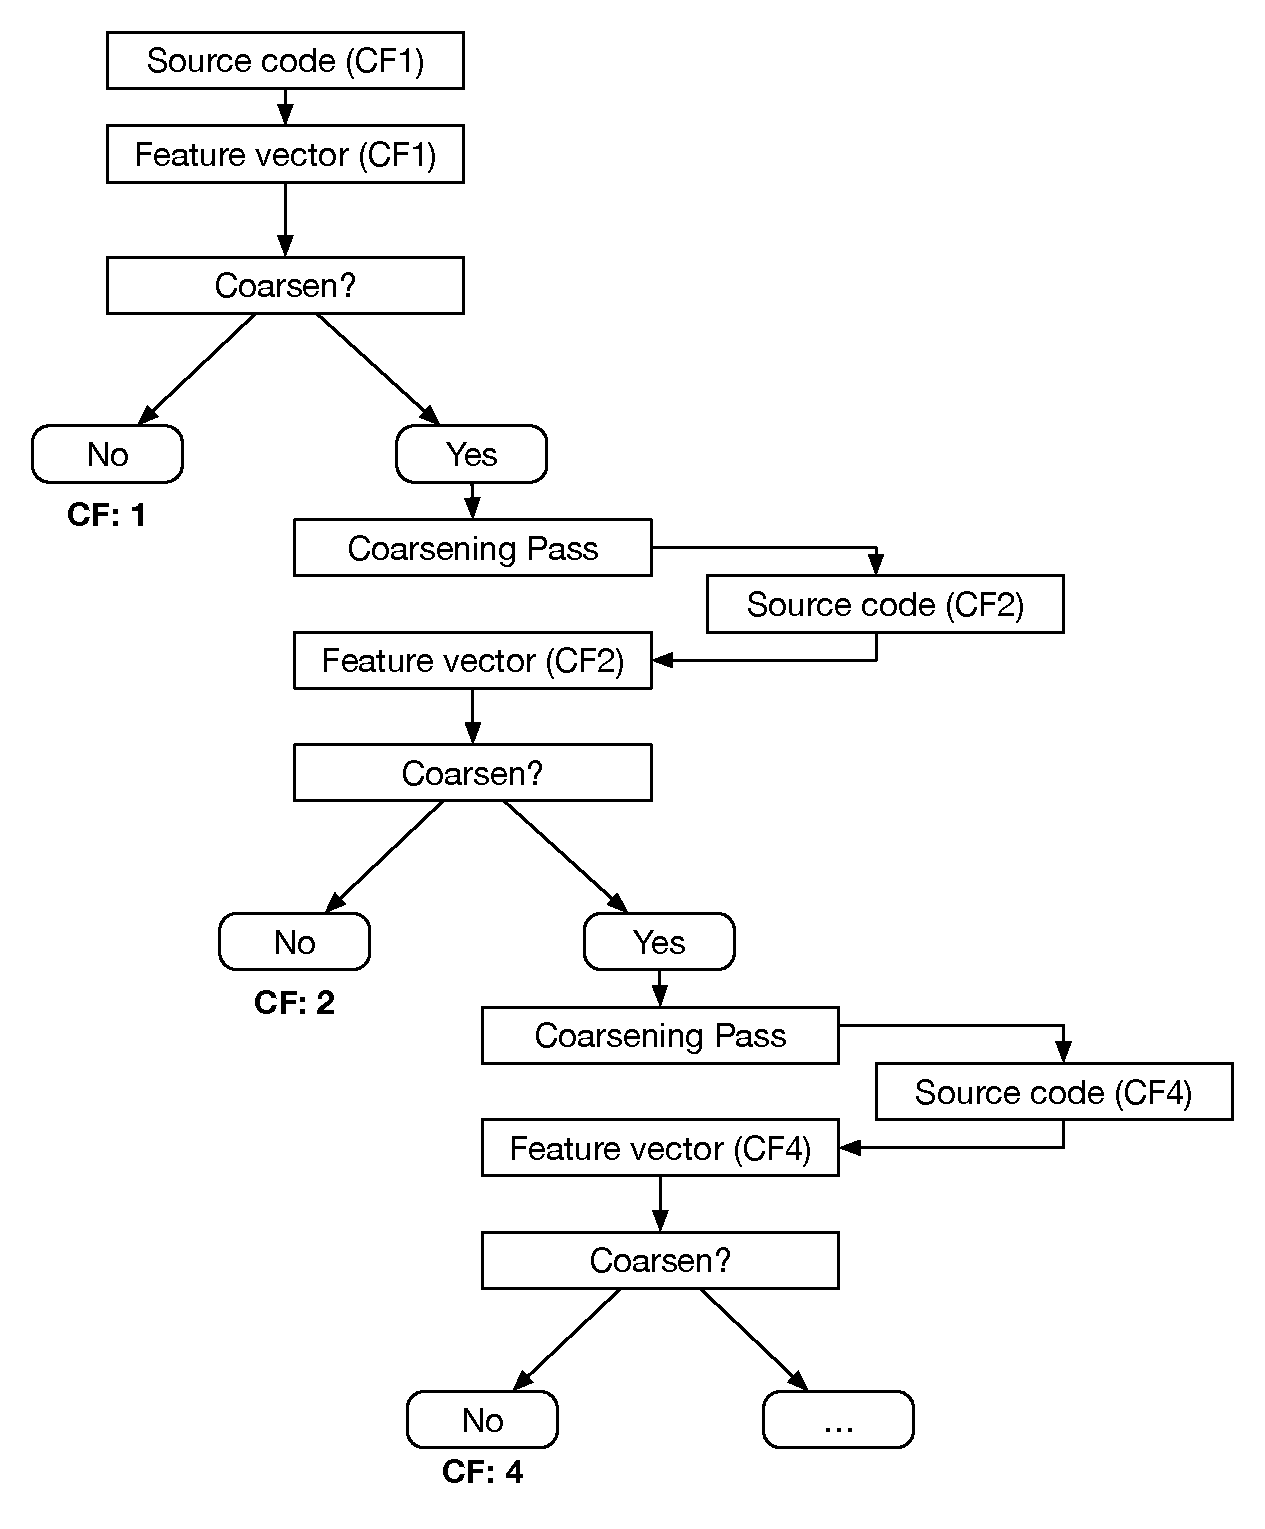
\includegraphics[width=.92\columnwidth]{img/cf-magni}%
    \label{fig:cf-magni}
  }\\*%
  \subfloat[Proposed approach.]{%
      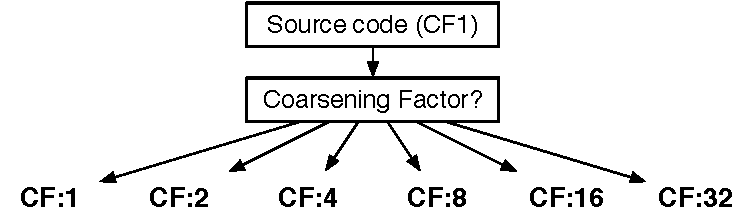
\includegraphics[width=.73\columnwidth]{img/cf-deeptune}%
      \label{fig:cf-deeptune}
  }%
  \caption[Predicting OpenCL thread coarsening factors.]{%
      Two approaches for predicting coarsening factor (CF) of OpenCL kernels.
      \citeauthor{Magni2014} reduce the multi-label classification problem to a
      series of binary decisions by iteratively applying the optimisation and
      computing new feature vectors. The proposed approach simply predicts the coarsening factor directly from the source code.%
  }
  \label{fig:cascading-nn}
\end{figure}

\begin{table}
  \rowcolors{2}{gray!25}{white}
  \centering%
    \begin{tabular}{| l l |}
      \hline
      \rowcolor{gray!50}
      \textbf{Name} & \textbf{Description} \\
      \hline
      \texttt{BasicBlocks} & \#.\ basic blocks \\
      \texttt{Branches} & \#.\ branches \\
      \texttt{DivInsts} & \#.\ divergent instructions \\
      \texttt{DivRegionInsts} & \#.\ instructions in divergent regions \\
      \texttt{DivRegionInstsRatio} & \#.\ instr. in divergent regions / total instructions \\
      \texttt{DivRegions} & \#.\ divergent regions \\
      \texttt{TotInsts} & \#.\ instructions \\
      \texttt{FPInsts} & \#.\ floating point instructions \\
      \texttt{ILP} & average ILP / basic block \\
      \texttt{Int/FP Inst Ratio} & \#.\ branches \\
      \texttt{IntInsts} & \#.\ integer instructions \\
      \texttt{MathFunctions} & \#.\ match builtin functions \\
      \texttt{MLP} & average MLP / basic block \\
      \texttt{Loads} & \#.\ loads \\
      \texttt{Stores} & \#.\ stores \\
      \texttt{UniformLoads} & \#.\ loads unaffected by coarsening direction \\
      \texttt{Barriers} & \#.\ barriers \\
      \hline
    \end{tabular}%
    \label{tab:features-pact14-raw}%
  \caption[\emph{Magni et al.\ }features for predicting thread coarsening]{%
    Candidate features used by \emph{Magni et al.\ }for predicting thread
    coarsening. From these values, they compute relative deltas for each
    iteration of coarsening, then use PCA for selection.%
  }%
  \label{tab:magni-features} %
\end{table}



\paragraph*{Expert Chosen Features}

\citeauthor{Magni2014} followed a comprehensive feature engineering process. 17 candidate features were assembled from previous studies of performance counters and computed theoretical values~\cite{Magni2,Sim2012}. For each candidate feature, they compute its coarsening \emph{delta}, reflecting the change in each feature value caused by coarsening: $f_{\Delta} = (f_{after} - f_{before}) / f_{before}$, adding it to the feature set. Then they use Principal Component Analysis (PCA) on the 34 candidates and selected the first 7 principal components, accounting for 95\% of variance in the space.


\subsection{Experimental Setup}

The experimental setup of \citeauthor{Magni2014}~\cite{Magni2014} is replicated for this case study. The thread coarsening optimisation is evaluated on 17 programs, listed in Table~\ref{tab:pact-benchmarks}. Four different GPU architectures are used, listed in Table~\ref{tab:pact-platforms}.

\begin{table}
  \centering %
  \rowcolors{2}{gray!25}{white}
  \begin{tabular}{| l r r r |}
    \hline
    \rowcolor{gray!50}
    & \textbf{Version} & \textbf{\#. benchmarks} & \textbf{\#. kernels}\\
    \hline
    \textbf{NVIDIA SDK} & 4.2 & 3 & 3 \\
    \textbf{AMD SDK} & 3.0 & 10 & 10 \\
    \textbf{Parboil~\cite{Stratton2012}} & 0.2 & 4 & 4 \\
    \textbf{Total} & - & 17 & 17 \\
    \hline
  \end{tabular}
  \caption[Benchmarks used in Case Study B]{%
    Benchmarks used in Case Study B.%
  }
  \label{tab:pact-benchmarks}
\end{table}

\begin{table}[t!]
  \centering %
  \rowcolors{2}{gray!25}{white}
  \begin{tabular}{| l l l l |}
    \hline
    \rowcolor{gray!50}
    & \textbf{Frequency} & \textbf{Memory} & \textbf{Driver} \\
    \hline
    \textbf{AMD HD 5900} & 725 MHz & 2GB & AMD 1124.2 \\
    \textbf{AMD Tahiti 7970} & 1000 MHz & 3GB & AMD 1084.4 \\
    \textbf{NVIDIA GTX 480} & 700 MHz & 1536 MB & NVIDIA 304.54 \\
    \textbf{NVIDIA K20c} & 706 MHz & 5GB & NVIDIA 331.20 \\
    \hline
  \end{tabular}
  \caption[Experimental platforms used in Case Study B]{%
    Experimental platforms used in Case Study B.%
  }
  \label{tab:pact-platforms}
\end{table}


\paragraph*{DeepTune Configuration}

Figure~\ref{fig:nn}b shows the artificial neural network configuration. The OpenCL kernel is the sole input and coarsening factor is the predicted output.


\paragraph*{Model Evaluation}

Compared to Case Study A, the size of the evaluation is small. As such, \emph{leave-one-out cross-validation} is used to evaluate the models. For each program, a model is trained on data from all other programs and used to predict the coarsening factor of the excluded program.

The parameters of the artificial neural network are not described in~\cite{Magni2014}, so an additional, \emph{nested} cross-validation process is used to find the optimal model parameters. For every program in the training set, a grid search of 48 combinations of network parameters is performed. The best performing parameter configuration is selected from these 768 results to train a model for prediction on the excluded program. This nested cross-validation is repeated for each of the training sets. No such tuning of hyper-parameters is performed for DeepTune.


\subsection{Comparison to Case Study A}

For the two different optimisation heuristics, the authors arrived at very different predictive model designs, with very different features. By contrast, the DeepSmith approach is exactly the same for both problems. None of DeepTune's parameters were tuned for the case studies presented above. Their settings represent conservative choices expected to work reasonably well for most scenarios.

Table~\ref{tab:nn-size} shows the similarity of the models. The only difference between the network designs is the auxiliary inputs for Case Study A and the different number of optimisation decisions. The differences between DeepTune configurations is only two lines of code: the first, adding the two auxiliary inputs; the second, increasing the size of the output layer for Case Study B from two neurons to six. The description of these differences is larger than the differences themselves.

\begin{table}
  \centering
  \rowcolors{2}{white}{gray!25}
  \begin{tabular}{| l r r | r r |}
    \hline
    \rowcolor{gray!50}
    & \multicolumn{2}{c}{\textbf{\#.\ neurons}} & \multicolumn{2}{c}{\textbf{\#.\ parameters}} \\
    \rowcolor{gray!50}
    & \textbf{HM} & \textbf{CF} & \textbf{HM} & \textbf{CF} \\
    \hline
    \textbf{Embedding} & 64 & 64 & ,256 & 8,256 \\
    \textbf{LSTM\_1} & 64 & 64 & 33,024 & 33,024 \\
    \textbf{LSTM\_2} & 64 & 64 & 33,024 & 33,024 \\
    \textbf{Concatenate} & 64 + 2 & - & - & - \\
    \textbf{Batch Normalisation} & 66 & 64 & 264 & 256 \\
    \textbf{DNN\_1} & 32 & 32 & 2,144 & 2,080 \\
    \textbf{DNN\_2} & 2 & 6 & 66 & 198 \\
    \hline
    \textbf{Total} & & & 76,778 & 76,838 \\
    \hline
  \end{tabular}
  \caption[DeepTune model parameters]{%
    The size and number of parameters of the DeepTune components of
    Figure~\ref{fig:nn}, configured for heterogeneous mapping (HM) and
    coarsening factor (CF).%
  }
  \label{tab:nn-size}
\end{table}



\subsection{Experimental Results}

Exploiting thread coarsening for OpenCL kernels is a difficult task. On average, coarsening slows programs down. The speedup attainable by a perfect heuristic is only $1.36\times$.

Figures~\ref{fig:pact-speedup-left} and~\ref{fig:pact-speedup-right} show speedups achieved by the \citeauthor{Magni2014} and DeepTune models for all programs and platforms. The performance of programs without coarsening is used as a baseline. On the four experimental platforms (AMD HD 5900, Tahiti 7970, NVIDIA GTX 480, and Tesla K20c), the \citeauthor{Magni2014} model achieves average speedups of $1.21\times$, $1.01\times$, $0.86\times$, and $0.94\times$, respectively. DeepTune outperforms this, achieving speedups of $1.10\times$, $1.05\times$, $1.10\times$, and $0.99\times$.

Some programs --- especially those with large divergent regions or indirect memory accesses --- respond poorly to coarsening. No performance improvement is possible on the \texttt{mvCoal} and \texttt{spmv} programs. Both models fail to achieve positive average speedups on the NVIDIA Tesla K20c, because thread coarsening does not give performance gains for the majority of the programs on this platform.

The disappointing results for both predictive models may be attributed to the small training program set (only 17 programs in total). As a result, the models suffer from sparse training data. In Chapter~\ref{chap:clgen} of this thesis, a methodology for overcoming data sparsity using additional programs is presented. In this instance, the shared structure of the DeepTune models between the two case studies enables an alternative strategy to overcome data scarcity. The following subsection describes and tests a novel strategy for training optimisation heuristics on a small number of programs by exploiting knowledge learned from other optimisation domains.

\begin{figure}
  \centering %
  \subfloat[][]{%
    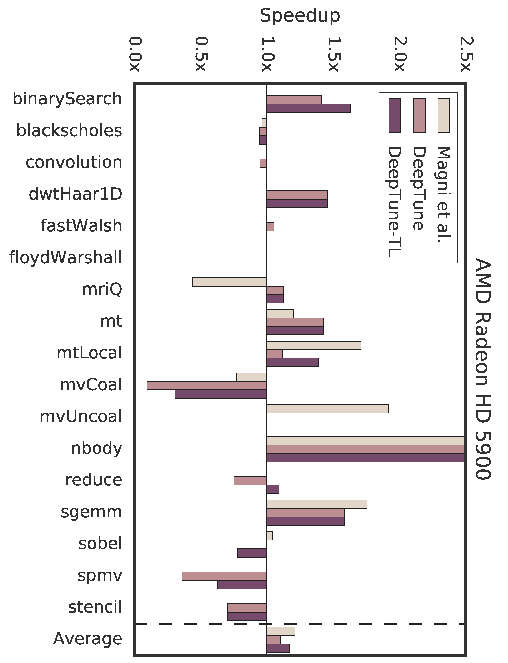
\includegraphics[width=.6\columnwidth,angle=90]{img/pact-speedup-a}%
    \label{fig:pact-speedup-a}%
  }%
  \\*
  \subfloat[][]{%
    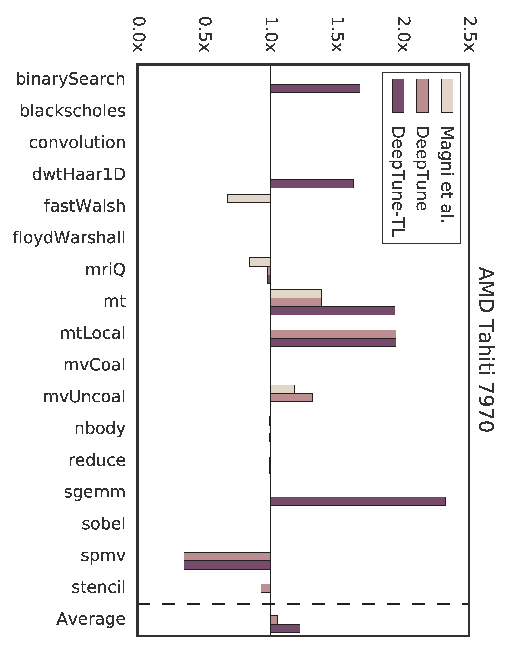
\includegraphics[width=.6\columnwidth,angle=90]{img/pact-speedup-b}%
    \label{fig:pact-speedup-b}%
  }%
  \caption[Speedups of predicted thread coarsening factors on AMD]{%
    Speedups of predicted coarsening factors on AMD platforms. DeepTune outperforms \citeauthor{Magni2014} on three of the four platforms. Transfer learning improves DeepTune speedups further, by 16\% on average.%
  }%
  \label{fig:pact-speedup-left}
\end{figure}

\begin{figure}
  \centering %
  \subfloat[][]{%
    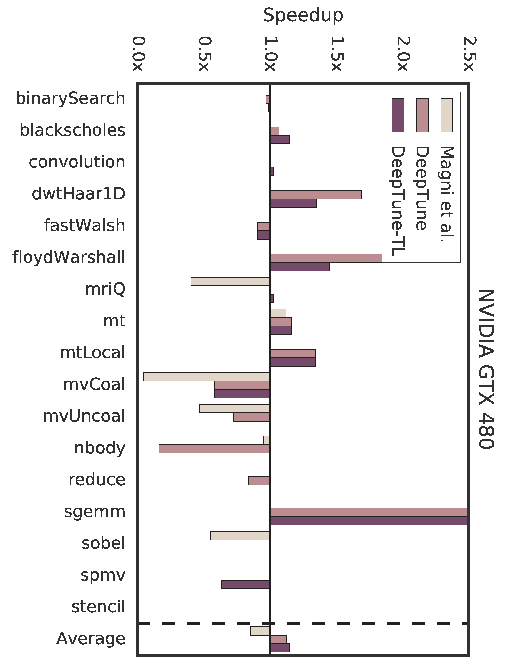
\includegraphics[width=.6\columnwidth,angle=90]{img/pact-speedup-c}%
    \label{fig:pact-speedup-c}%
  }%
  \\*
  \subfloat[][]{%
    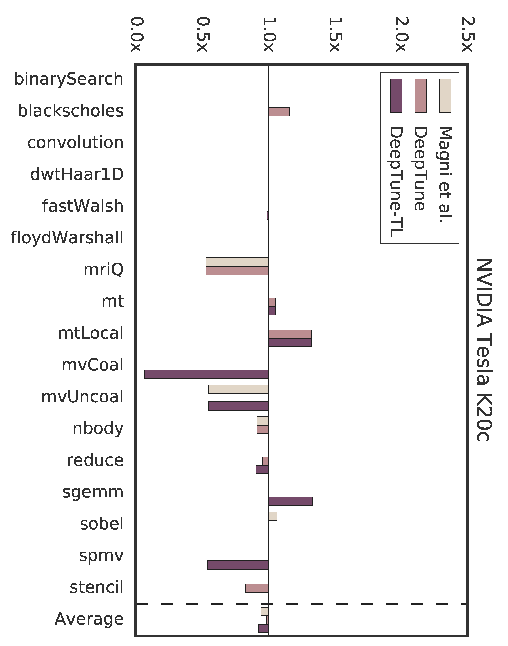
\includegraphics[width=.6\columnwidth,angle=90]{img/pact-speedup-d}%
    \label{fig:pact-speedup-d}%
  }%
  \caption[Speedups of predicted thread coarsening factors on NVIDIA]{%
    Speedups of predicted coarsening factors on NVIDIA platforms. DeepTune outperforms \citeauthor{Magni2014} on three of the four platforms. Transfer learning improves DeepTune speedups further, by 16\% on average.%
  }%
  \label{fig:pact-speedup-right}
\end{figure}


\section{Transfer Learning Across Problem Domains}
\label{sec:deeptune-transfer-learning}

There are inherent differences between the tasks of building heuristics for heterogeneous mapping and thread coarsening, evidenced by the contrasting choices of features and models used by the state-of-the-art approaches in Case Studies A and B. However, in both cases, the first role of DeepTune is to extract meaningful abstractions and representations of OpenCL code. Prior research in deep learning has shown that models trained on similar inputs for different tasks often share useful commonalities. The idea is that in classification using artificial neural networks, information learned at the early layers of artificial neural networks (i.e. closer to the input layer) will be useful for multiple tasks. The later the network layers are (i.e. closer to the output layer), the more specialised the layers become~\cite{Zeiler2014}.

Hypothesising that this would be the case for DeepTune would enable the novel transfer of information \emph{across different optimisation domains}. To test this, the language model --- the \texttt{Embedding}, and \texttt{LSTM\_\{1,2\}} layers --- trained for the heterogeneous mapping task was extracted and \emph{transferred} over to the new task of thread coarsening. Since DeepTune keeps the same design for both optimisation problems, this is as simple as copying the learned parameters of the three layers. The model is then trained as normal.

As shown in Figures~\ref{fig:pact-speedup-left} and~\ref{fig:pact-speedup-right}, the newly trained model, DeepTune-TL has improved performance for 3 of the 4 platforms: $1.17\times$, $1.23\times$, $1.14\times$, $0.93\times$, providing an average 12\% performance improvement over \citeauthor{Magni2014}. In 81\% of cases, the use of transfer learning matched or improved the optimisation decisions of DeepTune, providing up to a 16\% improvement in per platform performance.

On the NVIDIA Tesla K20c, the platform for which no predictive model achieves positive average speedups, DeepTune-TL matches or improve performance in the majority of cases, but over-coarsening on three of the programs causes a modest reduction in average performance. For this platform, further performance results are suspected necessary due to its unusual optimisation profile.


\section{DeepTune Internal Activation States}
\label{sec:deeptune-internal-states}

\begin{figure}
  \centering %
  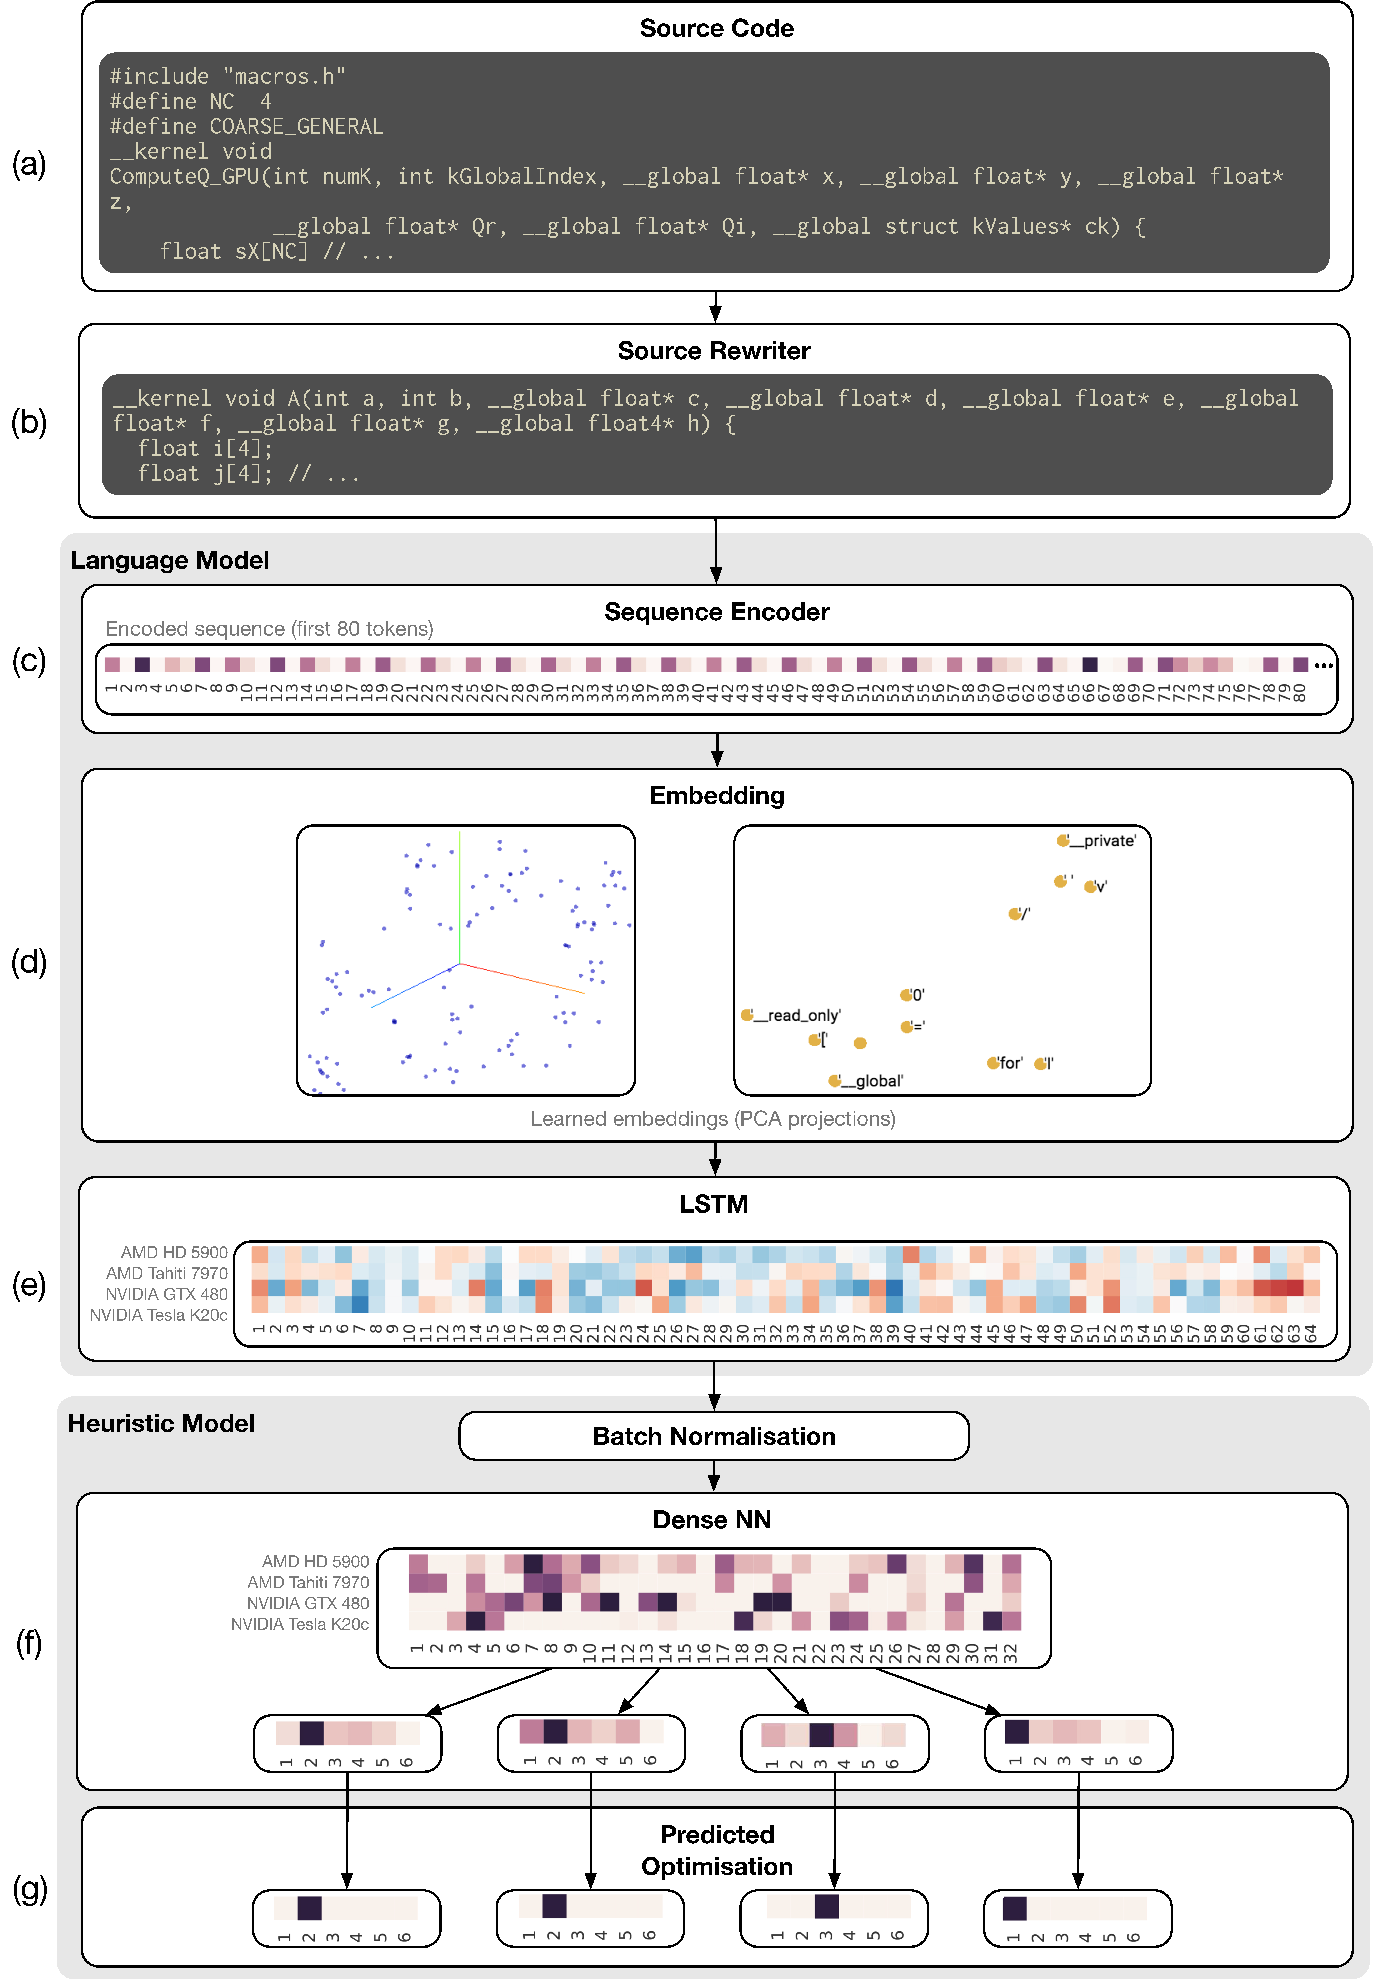
\includegraphics[width=\textwidth]{img/viz}%
  \caption[Visualising the internal state of DeepTune]{%
    Visualising the internal state of DeepTune when predicting coarsening factor for Parboil's \texttt{mriQ} benchmark on four different architectures. The activations in each layer of the four models increasingly diverge the lower down the network.%
  }
  \label{fig:viz} %
\end{figure}

In previous sections, DeepTune is shown to automatically outperform state-of-the-art predictive models for which experts have invested a great amount of time in engineering features. This section attempts to illuminate the inner workings, using a single example from Case Study B: predicting the thread coarsening factor for Parboil's \texttt{mriQ} benchmark on four different platforms.

Figure~\ref{fig:viz} shows the DeepTune configuration, with visual overlays showing the internal state. From top to bottom, the input to the model is the 267 lines of OpenCL code for the \texttt{mriQ} kernel. This source code is preprocessed, formatted, and rewritten using variable and function renaming, shown in Figure~\ref{fig:viz}b. The rewritten source code is tokenised and encoded in a $1$-of-$k$ vocabulary. Figure~\ref{fig:viz}c shows the first 80 elements of this encoded sequence as a heat map in which each cell's colour reflects its encoded value. The input, rewriting, and encoding is the same for each of the four platforms.

The encoded sequences are then passed into the Embedding layer. This maps each token of the vocabulary to a point in a 64 dimension vector space. Embeddings are learned during training so as to cluster semantically related tokens together. As such, they may differ between the four platforms. Figure~\ref{fig:viz}d shows a 3-dimensional PCA projection of the embedding space for one of the platforms, showing multiple clusters of tokens. Although achieving good separation of embedding clusters typically requires a much larger training set~\cite{Ben-nun2018}, by honing in on one of the clusters and annotating each point with its corresponding token, it can be observed that the cluster contains the semantically related OpenCL address space modifiers \texttt{\_\_private}, \texttt{\_\_global}, and \texttt{\_\_read\_only}.

Two layers of 64 LSTM neurons model the sequence of embeddings, with the neuron activations of the second layer being used to characterise the entire sequence. Figure~\ref{fig:viz}e shows the neurons in this layer for each of the four platforms, using a red-blue heat map to visualise the intensity of each activation. Comparing the activations between the four platforms reveals a number of neurons in the layer with different responses across platforms. This indicates that the language model is partly specialised to the target platform. Subsequent work~\cite{Ben-nun2018} supports this reasoning, in which performance is slightly degraded by training parts of the language model in a platform-agnostic manner.

As information flows through the network, the layers become progressively more specialised to the specific platform. This can be seen in Figure~\ref{fig:viz}f, which shows the two layers of the heuristic model. The activations within these increasingly diverge. The mean variance of activations across platforms increases threefold compared to the language model, from 0.039 to 0.107. Even the activations of the AMD HD 5900 and AMD Tahiti 7970 platforms are dissimilar, despite the final predicted coarsening factor for both platforms being the same. The largest activation of the output layer is taken in Figure~\ref{fig:viz}g as the final predicted coarsening factor. For this particular program, a state-of-the-art model achieves 54\% of the maximum performance. DeepTune achieves 99\%.


\section{Summary}
\label{sec:deeptune-conclusion}

Applying machine learning to compiler and runtime optimisations requires generating features first. This is a time-consuming process, it needs supervision by an expert, and even then one cannot be sure that the selected features are optimal. This \emph{feature design} challenge (Section~\ref{subsec:challenge-features}) places a significant burden on developers looking to adopt machine learning for constructing compiler optimisation heuristics. This chapter presents a novel tool for building optimisation heuristics, DeepTune, which forgoes feature extraction entirely, relying on powerful language modelling techniques to automatically build effective representations of programs directly from raw source code. The result translates into a huge reduction in development effort, improved heuristic performance, and simpler model designs.

The approach is fully automated. Using DeepTune, developers no longer need to spend months using statistical methods and profile counters to select program features via trial and error. It is worth mentioning that the model design or parameters are not tailored for the optimisation task at hand, yet DeepTune achieves performance on par with and in most cases \emph{exceeding} state-of-the-art predictive models.

In this chapter, DeepTune is used to automatically construct heuristics for two challenging compiler and runtime optimisation problems. In both cases, DeepTune is found to outperform state-of-the-art predictive models by 14\% and 12\%. The DeepTune architecture is shown also to allow the exploitation of information learned from another optimisation problem to give the learning a boost. Doing so provides up to a 16\% performance improvement when training using a handful of programs. This approach may prove useful in other domains for which training data are a scarce resource.
